%%%%%%%%%%%%%%%%%%%%%%%%%%%%%%%%%%%%%%%
\subsection{External Neutron Source}\label{sec:neutron}
%Primary// secondary purpose like above, but direct test of neutron response model.  (nice for TP?) 
In a \dword{lartpc}, for a fixed amount of ionization deposited at a point in the detector, the amount of charge produced and collected depends on several factors such as argon purity, electron lifetime, noise, and strength of E-field. Given these factors, it is highly desirable to have a ``standard candle'' energy deposition of known energy that can be detected throughout the volume. Such a standard deposition would reveal variations in the local electron collection efficiency, especially if the source could be triggered such that the $t_0$ of the interaction was known. %Examples of such systems include external deployment of radioactive sources of known energy as discussed in Section~\ref{sec:rs} and direct injection of short-lived radioactive atoms into the \dword{lar}.
%Another such system is the external neutron generator system.
An external neutron generator system would be a triggered, known charge source.

%%%%%%%%%%%%%%%%%%%%%
\subsubsection{Motivation and Possible Measurements}

%A neutron system provides

%In a %TPC 
%\dword{lartpc},
%the energy reconstruction of a track depends on the amount of charge detected from electrons drifting from the track to the collection plane. 
%for a fixed amount of ionization deposited at a point in the detector, the amount of charge produced and collected depends on several factors such as argon purity, electron lifetime, noise, and strength of E-field.
%$$$$
%SG: too repetitive of what was covered in David's section and intro etc. so exclude it.
%$$$$
%\begin{enumerate}
%\item The local electric field strength affects the fraction of charge that recombines before drifting. As the field increases % The stronger the field, the 
%less immediate recombination takes place, and thus the ratio of drifting electrons to energy deposited increases.
%\item The electron lifetime depends strongly on the purity of the \dword{lar}. Given the large size of %the DUNE TPC, 
%each \dword{detmodule} the restrictions on the flow in the active volume, and a likely temperature gradient inside the liquid, %it can be expected that 
%there will likely be parts of the detector where the electron lifetime is shorter than others. The prediction of exactly how this manifests is difficult to predict {\it ab initio}.
%\item The distance electronics have to drift% to be collected 
%before collection depends on the location of the vertex inside the volume. The longer the drift, the more likely it is an electron will be absorbed.
%\item Some parts of the detector %can in principle 
%may be better or worse than others in terms of noise. This can affect the threshold charge collection systematically for different areas or the detector.
%\end{enumerate}

%Given these factors, it is highly desirable to %be able to have a ``standard candle'' energy deposition of known energy that can be detected throughout the volume. Such a standard deposition would reveal variations in the local electron collection efficiency, especially if the source could be triggered such that the $t_0$ of the interaction was known. Examples of such systems include external deployment of radioactive sources of known energy as discussed in Section~\ref{sec:rs} and direct injection of short-lived radioactive atoms into the \dword{lar}. 

%$$$$$$
%SG:Remove. Works against Juergen's system. TP is not the place to compete b/n various sytems. All systems have short comings that can't be the motivation. Motivation has to be physics
%$$$$$$
%In principle, radioactive sources of known energy distribution could be deployed throughout the detector, but there are several problems with this approach: (1)  the source must be physically placed at the desired point, % one wishes to check, 
%requiring multiple deployments in order to sample a significant volume of the detector, (2) the presence of the source itself can alter the electric field and ionization yield, and (3) the introduction of a foreign object into the active volume of the detector carries the risk of introducing impurities and/or radioactive contaminants. In addition, in order to have a triggered source (and hence some idea of $t_0$), %one would have 
%it would be necessary to introduce trigger electronics or other instrumentation -- further complicating the deployment and increasing the risk.

%A way around this dilemma is to introduce short-lived radioactive atoms into the \dword{lar} itself, but this has the disadvantage that there is no trigger and no way to ensure that the standard candle decays spread out through the whole volume. In addition, to be useful, such isotopes would have to have appreciable half-lives in order to have time to spread around the detector, and thus the whole process might take many hours. Finally, such isotopes would likely need to be made locally, which can be expensive and difficult.

%One way around these 
%One could avoid these issues by % is to take 
The neutron generator system takes advantage of a remarkable property of argon -- the near transparency to neutrons with an energy near \SI{57}{\keV} due to an anti-resonance in the cross section caused by the destructive interference between two high-level states of the \isotope{Ar}{40} nucleus. As shown in Figure~\ref{fig:Arxsec}, this cross section is about \SI{10}{\keV} wide, and at the bottom the cross section of \num{1.6e-4} %$1.6\times 10^{-4}\; b$ 
implies an elastic scattering length of over \SI{2000}{\m}. Thus to neutrons of this energy the DUNE \dword{lartpc} % TPC 
is essentially transparent, and if injected from the top of the detector, would reach every part of the active volume. Of course, natural argon has three major isotopes: \isotope{Ar}{36} (0.3336\%), \isotope{Ar}{38} (0.0834\%), and \isotope{Ar}{40} (99.6035\%) each with a slightly different anti-resonance. \fixme{(NOTE: PUT IN EFFECTIVE CROSS SECTION)}

\begin{dunefigure}[Elastic scattering cross sections on argon isotopes]{fig:Arxsec}
{Elastic scattering cross sections on \isotope{Ar}{40} (top left), \isotope{Ar}{36} (top right), and \isotope{Ar}{38} (bottom). From ENDF/B-VII.1~\cite{ref:ENDF}. The large anti-resonance at $57\; keV$ in 40-Ar can be clearly seen.}
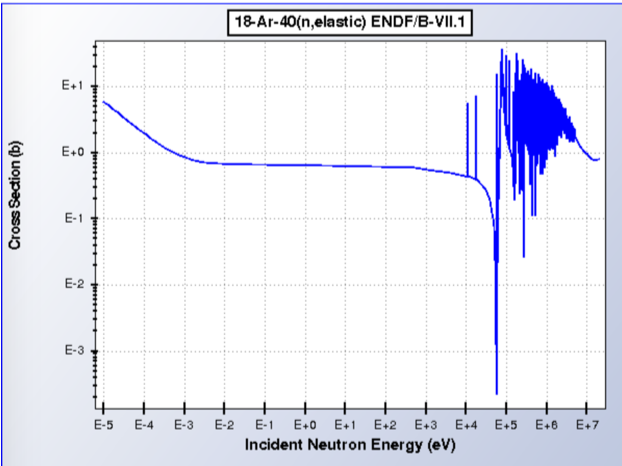
\includegraphics[width=0.4\linewidth]{Ar40xsec.png}
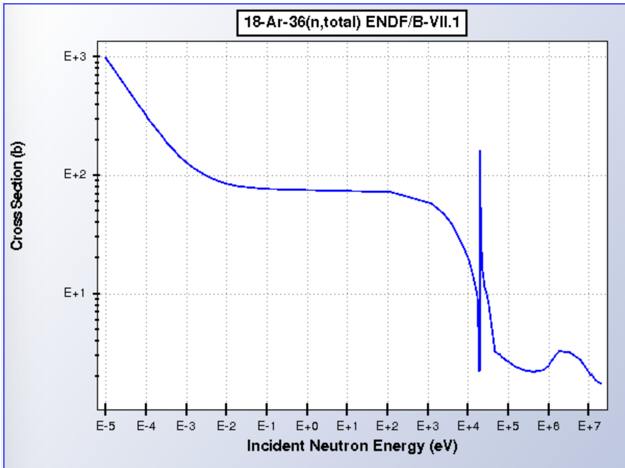
\includegraphics[width=0.4\linewidth]{Ar36xsec.png}
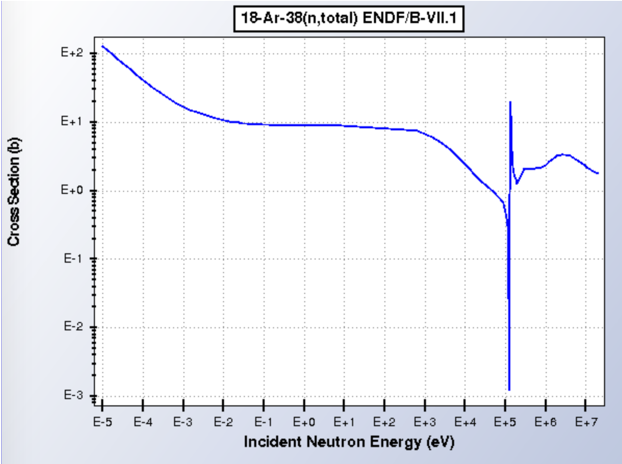
\includegraphics[width=0.4\linewidth]{Ar38xsec.png}
\end{dunefigure}
\fixme{NOTE: PUT IN PLOTS FOR ELASTIC}
\fixme{Resolution of plots too bad and labels/titles not readable; get updated plots}

Those that do scatter lose energy, leave the anti-resonance (where the scattering length is about \SI{70}{\cm}), quickly slow down and are captured. Each capture releases exactly the binding energy difference between \isotope{Ar}{40} and \isotope{Ar}{41}, about \SI{6.1}{\MeV} in the form of gamma rays.  As will be described below, by using a {\it DD Generator}\footnote{{\it DD} stands for "Deuterium-Deuterium" }, a triggered pulse of neutrons can be generated outside the TPC, then injected via a dedicated hole in the insulation into the \dword{lar}, where is spreads through the entire volume to produce ``standard candle'' \SI{6.1}{\MeV} energy depositions. Using this method, 
%SG:competing with other systems
%there would be no need for internal deployments, 
the calibration procedure would be quick (likely less than 30 minutes).
%, and there is no need to manufacture short-lived isotopes at an external facility.

\begin{dunefigure}[h]{fig:Arxsec2}{Total scattering cross sections on 40-Ar in the range $10-200\; keV$~\cite{ref:ENDF}}
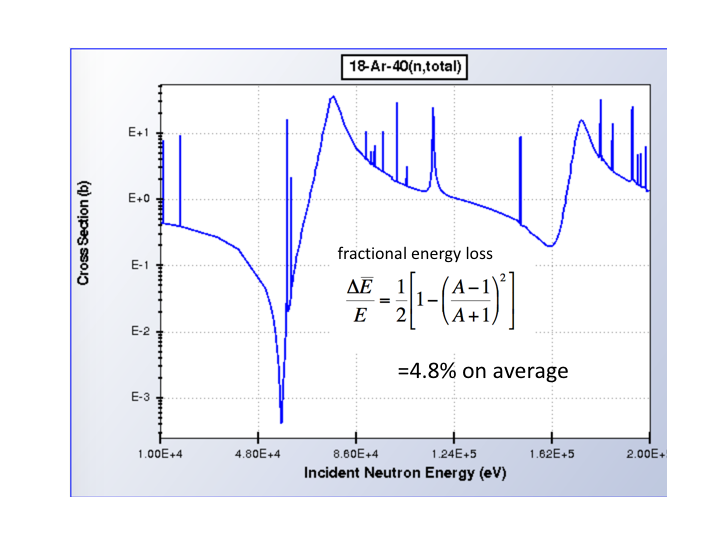
\includegraphics[width=0.75\linewidth]{Ar40Xsec2.png}
\end{dunefigure}

A relevant question is what fraction of neutrons slowing down from higher energy will fall into the anti-resonance. Figure~\ref{fig:Arxsec2} shows an expanded view of the total \isotope{Ar}{40} cross section in the range  \num{10} to \SI{200}{\keV}. Since the average energy loss of a neutron elastically scattering off a \isotope{Ar}{40} nucleus is \num{4.8}\%, in the region of the anti-resonance the average energy loss per scatter is about \SI{3}{\keV}. Therefore, estimating the width of the anti-resonance to be about \SI{10}{\keV}, a large fraction of the neutrons injected can be expected to fall into the cross section hole. Indeed, as will be shown in preliminary simulations, many neutrons scatter several times before escaping to lower energies to be captured. This simple phenomenon tends to scatter neutrons isotropically around the \dword{lar}.

The neutron capture gamma spectrum is also being characterized. In Nov 2017, the ACED Collaboration took several hundred thousand neutron capture events at the DANCE facility at LANSCE which will be used to prepare a database of the neutron capture gamma cascade chain.

%%%%%%%%%%%%%%%%%%%%%
\subsubsection{Design Considerations} 

%Figure~\ref{fig:PDLayout} shows a conceptual layout of the neutron injection system.

The fixed, shielded $DD$ generator would be located above a feedthrough in the hydrogenous insulation. Pulsed\footnote{The pulse width is \SI{100}{\micro\s}, but it is possible to reduce this by simply shortening the \dword{hv} pulse that sustains the reaction.}, commercially available $DD$ generators exist and are cost competitive. Between the generator and the cryostat, layers of water or plastic and intermediate fillers will be included for sufficient degradation of the neutron energy. Initial simulations indicate that a single neutron injection point would illuminate %all of ProtoDUNE's volume.
the entire volume of one of the \dword{protodune} detectors. The $DD$ generator itself is the size of a large thermos bottle. Space needed by the system will be determined by the desired shielding level which is yet to be understood.

%%%%%%%%%%%%%%%%%%%%%
\subsubsection{Remaining Studies}

The remaining studies for the TDR for the external neutron source are:
\begin{itemize}
%SG: No need to include these details in TP; need to check with cryostat engineers.
%\item ?? \fixme{Feedthrough collision? Where are we putting this and aren't the rest spoken for? Can we place and remove it with other radioactive sources? }
\item Assessment of the full design, including degrader materials and shielding.
\item Assessment of sufficient space and mounting (weight) considerations above the cryostat considering shielding for the neutron generator. 
\end{itemize}

\fixme{add more studies}

